
\documentclass[letterpaper,hide notes,xcolor={table,svgnames},pdftex]{beamer}
\def\showexamples{t}


%\usepackage[svgnames]{xcolor}

%% Demo talk
%\documentclass[letterpaper,notes=show]{beamer}

\usecolortheme{crane}
\setbeamertemplate{navigation symbols}{}

\usetheme{MyPittsburgh}
%\usetheme{Frankfurt}

%\usepackage{tipa}

\usepackage{hyperref}
\usepackage{graphicx,xspace}
\usepackage[normalem]{ulem}

\newcommand\SF[1]{$\bigstar$\footnote{SF: #1}}



\newcounter{tmpnumSlide}
\newcounter{tmpnumNote}

% old question code
%\newcommand\question[1]{{$\bigstar$ \small \onlySlide{2}{#1}}}
% \newcommand\nquestion[1]{\ifdefined \presentationonly \textcircled{?} \fi \note{\par{\Large \textbf{?}} #1}}
% \newcommand\nanswer[1]{\note{\par{\Large \textbf{A}} #1}}


 \newcommand\mnote[1]{%
   \addtocounter{tmpnumSlide}{1}
   \ifdefined\showcues {~\tiny\fbox{\arabic{tmpnumSlide}}}\fi
   \note{\setlength{\parskip}{1ex}\addtocounter{tmpnumNote}{1}\textbf{\Large \arabic{tmpnumNote}:} {#1\par}}}

\newcommand\mmnote[1]{\note{\setlength{\parskip}{1ex}#1\par}}

%\newcommand\mnote[2][]{\ifdefined\handoutwithnotes {~\tiny\fbox{#1}}\fi
% \note{\setlength{\parskip}{1ex}\textbf{\Large #1:} #2\par}}

%\newcommand\mnote[2][]{{\tiny\fbox{#1}} \note{\setlength{\parskip}{1ex}\textbf{\Large #1:} #2\par}}

\newcommand\mquestion[2]{{~\color{red}\fbox{?}}\note{\setlength{\parskip}{1ex}\par{\Large \textbf{?}} #1} \note{\setlength{\parskip}{1ex}\par{\Large \textbf{A}} #2\par}\ifdefined \presentationonly \pause \fi}

\newcommand\blackboard[1]{%
\ifdefined   \showblackboard
  {#1}
  \else {\begin{center} \fbox{\colorbox{blue!30}{%
         \begin{minipage}{.95\linewidth}%
           \hspace{\stretch{1}} Some space intentionally left blank; done at the blackboard.%
         \end{minipage}}}\end{center}}%
         \fi%
}



%\newcommand\q{\tikz \node[thick,color=black,shape=circle]{?};}
%\newcommand\q{\ifdefined \presentationonly \textcircled{?} \fi}

\usepackage{listings}
\lstset{%
  keywordstyle=\bfseries,
  aboveskip=15pt,
  belowskip=15pt,
  captionpos=b,
  identifierstyle=\ttfamily,
  escapeinside={(*@}{@*)},
  stringstyle=\ttfamiliy,
  frame=lines,
  numbers=left, basicstyle=\scriptsize, numberstyle=\tiny, stepnumber=0, numbersep=2pt}

\usepackage{siunitx}
\newcommand\sius[1]{\num[group-separator = {,}]{#1}\si{\micro\second}}
\newcommand\sims[1]{\num[group-separator = {,}]{#1}\si{\milli\second}}
\newcommand\sins[1]{\num[group-separator = {,}]{#1}\si{\nano\second}}
\sisetup{group-separator = {,}, group-digits = true}

%% -------------------- tikz --------------------
\usepackage{tikz}
\usetikzlibrary{positioning}
\usetikzlibrary{arrows,backgrounds,automata,decorations.shapes,decorations.pathmorphing,decorations.markings,decorations.text}

\tikzstyle{place}=[circle,draw=blue!50,fill=blue!20,thick, inner sep=0pt,minimum size=6mm]
\tikzstyle{transition}=[rectangle,draw=black!50,fill=black!20,thick, inner sep=0pt,minimum size=4mm]

\tikzstyle{block}=[rectangle,draw=black, thick, inner sep=5pt]
\tikzstyle{bullet}=[circle,draw=black, fill=black, thin, inner sep=2pt]

\tikzstyle{pre}=[<-,shorten <=1pt,>=stealth',semithick]
\tikzstyle{post}=[->,shorten >=1pt,>=stealth',semithick]
\tikzstyle{bi}=[<->,shorten >=1pt,shorten <=1pt, >=stealth',semithick]

\tikzstyle{mut}=[-,>=stealth',semithick]

\tikzstyle{treereset}=[dashed,->, shorten >=1pt,>=stealth',thin]

\usepackage{ifmtarg}
\usepackage{xifthen}
\makeatletter
% new counter to now which frame it is within the sequence
\newcounter{multiframecounter}
% initialize buffer for previously used frame title
\gdef\lastframetitle{\textit{undefined}}
% new environment for a multi-frame
\newenvironment{multiframe}[1][]{%
\ifthenelse{\isempty{#1}}{%
% if no frame title was set via optional parameter,
% only increase sequence counter by 1
\addtocounter{multiframecounter}{1}%
}{%
% new frame title has been provided, thus
% reset sequence counter to 1 and buffer frame title for later use
\setcounter{multiframecounter}{1}%
\gdef\lastframetitle{#1}%
}%
% start conventional frame environment and
% automatically set frame title followed by sequence counter
\begin{frame}%
\frametitle{\lastframetitle~{\normalfont(\arabic{multiframecounter})}}%
}{%
\end{frame}%
}
\makeatother

\makeatletter
\newdimen\tu@tmpa%
\newdimen\ydiffl%
\newdimen\xdiffl%
\newcommand\ydiff[2]{%
    \coordinate (tmpnamea) at (#1);%
    \coordinate (tmpnameb) at (#2);%
    \pgfextracty{\tu@tmpa}{\pgfpointanchor{tmpnamea}{center}}%
    \pgfextracty{\ydiffl}{\pgfpointanchor{tmpnameb}{center}}%
    \advance\ydiffl by -\tu@tmpa%
}
\newcommand\xdiff[2]{%
    \coordinate (tmpnamea) at (#1);%
    \coordinate (tmpnameb) at (#2);%
    \pgfextractx{\tu@tmpa}{\pgfpointanchor{tmpnamea}{center}}%
    \pgfextractx{\xdiffl}{\pgfpointanchor{tmpnameb}{center}}%
    \advance\xdiffl by -\tu@tmpa%
}
\makeatother
\newcommand{\copyrightbox}[3][r]{%
\begin{tikzpicture}%
\node[inner sep=0pt,minimum size=2em](ciimage){#2};
\usefont{OT1}{phv}{n}{n}\fontsize{4}{4}\selectfont
\ydiff{ciimage.south}{ciimage.north}
\xdiff{ciimage.west}{ciimage.east}
\ifthenelse{\equal{#1}{r}}{%
\node[inner sep=0pt,right=1ex of ciimage.south east,anchor=north west,rotate=90]%
{\raggedleft\color{black!50}\parbox{\the\ydiffl}{\raggedright{}#3}};%
}{%
\ifthenelse{\equal{#1}{l}}{%
\node[inner sep=0pt,right=1ex of ciimage.south west,anchor=south west,rotate=90]%
{\raggedleft\color{black!50}\parbox{\the\ydiffl}{\raggedright{}#3}};%
}{%
\node[inner sep=0pt,below=1ex of ciimage.south west,anchor=north west]%
{\raggedleft\color{black!50}\parbox{\the\xdiffl}{\raggedright{}#3}};%
}
}
\end{tikzpicture}
}


%% --------------------

%\usepackage[excludeor]{everyhook}
%\PushPreHook{par}{\setbox0=\lastbox\llap{MUH}}\box0}

%\vspace*{\stretch{1}

%\setbox0=\lastbox \llap{\textbullet\enskip}\box0}

\setlength{\parskip}{\fill}

\newcommand\noskips{\setlength{\parskip}{1ex}}
\newcommand\doskips{\setlength{\parskip}{\fill}}

\newcommand\xx{\par\vspace*{\stretch{1}}\par}
\newcommand\xxs{\par\vspace*{2ex}\par}
\newcommand\tuple[1]{\langle #1 \rangle}
\newcommand\code[1]{{\sf \footnotesize #1}}
\newcommand\ex[1]{\uline{Example:} \ifdefined \presentationonly \pause \fi
  \ifdefined\showexamples#1\xspace\else{\uline{\hspace*{2cm}}}\fi}

\newcommand\ceil[1]{\lceil #1 \rceil}


\AtBeginSection[]
{
   \begin{frame}
       \frametitle{Outline}
       \tableofcontents[currentsection]
   \end{frame}
}



\pgfdeclarelayer{edgelayer}
\pgfdeclarelayer{nodelayer}
\pgfsetlayers{edgelayer,nodelayer,main}

\tikzstyle{none}=[inner sep=0pt]
\tikzstyle{rn}=[circle,fill=Red,draw=Black,line width=0.8 pt]
\tikzstyle{gn}=[circle,fill=Lime,draw=Black,line width=0.8 pt]
\tikzstyle{yn}=[circle,fill=Yellow,draw=Black,line width=0.8 pt]
\tikzstyle{empty}=[circle,fill=White,draw=Black]
\tikzstyle{bw} = [rectangle, draw, fill=blue!20, 
    text width=4em, text centered, rounded corners, minimum height=2em]
    
    \newcommand{\CcNote}[1]{% longname
	This work is licensed under the \textit{Creative Commons #1 3.0 License}.%
}
\newcommand{\CcImageBy}[1]{%
	\includegraphics[scale=#1]{creative_commons/cc_by_30.pdf}%
}
\newcommand{\CcImageSa}[1]{%
	\includegraphics[scale=#1]{creative_commons/cc_sa_30.pdf}%
}
\newcommand{\CcImageNc}[1]{%
	\includegraphics[scale=#1]{creative_commons/cc_nc_30.pdf}%
}
\newcommand{\CcGroupBySa}[2]{% zoom, gap
	\CcImageBy{#1}\hspace*{#2}\CcImageNc{#1}\hspace*{#2}\CcImageSa{#1}%
}
\newcommand{\CcLongnameByNcSa}{Attribution-NonCommercial-ShareAlike}

\newenvironment{changemargin}[1]{% 
  \begin{list}{}{% 
    \setlength{\topsep}{0pt}% 
    \setlength{\leftmargin}{#1}% 
    \setlength{\rightmargin}{1em}
    \setlength{\listparindent}{\parindent}% 
    \setlength{\itemindent}{\parindent}% 
    \setlength{\parsep}{\parskip}% 
  }% 
  \item[]}{\end{list}} 




\title{Lecture 24 --- Software Lifecycle Models \& Tactics}

\author{Jeff Zarnett \& Patrick Lam \\ \small \texttt{jzarnett@uwaterloo.ca \& p.lam@ece.uwaterloo.ca}}
\institute{Department of Electrical and Computer Engineering \\
  University of Waterloo}
\date{\today}

\begin{document}

\begin{frame}
  \titlepage
\end{frame}

\part{Software Lifecycle Models}
\frame{\partpage}

\begin{frame}
\frametitle{Life Without Models}

\begin{center}
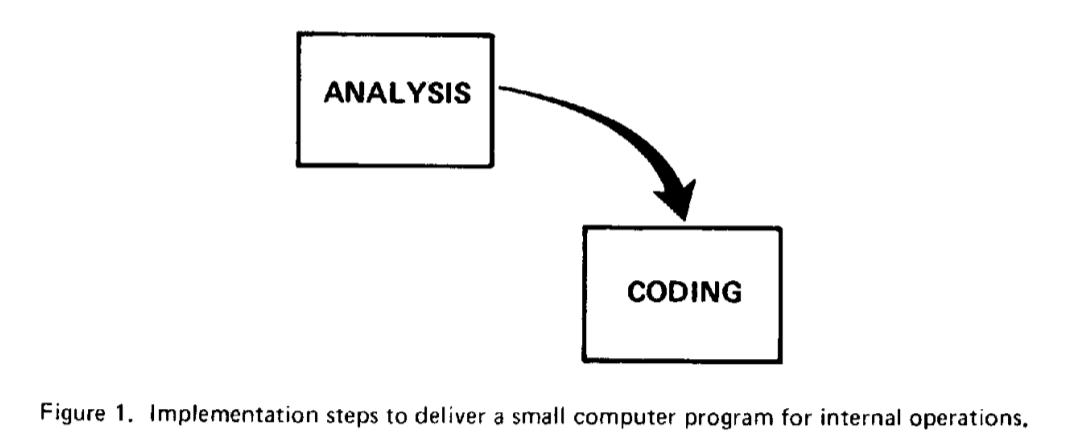
\includegraphics[height=.5\textheight]{images/two-stages.png}
\end{center}

from: Winston W. Royce. ``Managing the Development of Large Software Systems'', Proceedings IEEE WESCON, 1970.

\end{frame}

\begin{frame}
\frametitle{Deathmarches and Fiascoes}

\begin{changemargin}{1cm}
Software project management is hard.\\[1em]

\begin{center}
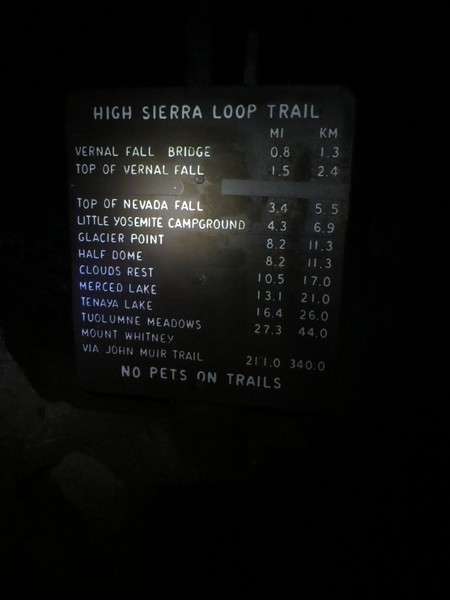
\includegraphics[width=.4\textwidth]{images/7897_trail_sign}
\end{center}

Software development lifecycle models try to avoid deathmarches and fiascoes.

\end{changemargin}
\end{frame}

\begin{frame}
\frametitle{Death Marches}

\begin{changemargin}{1cm}
Some amount of pressure in a project is normal.

When there is so much pressure that success is impossible, it's a \textit{Death March}.

Some possible causes:\\
\begin{itemize}
	\item Naive optimism
	\item Organizational politics
	\item Trying to build a huge project all at once
	\item Managerial incompetence
\end{itemize}
\end{changemargin}
\end{frame}


\begin{frame}
\frametitle{Iterations}
\begin{center}
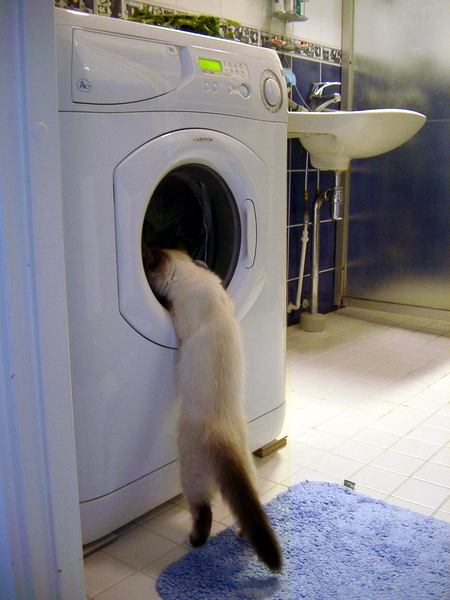
\includegraphics[width=.35\textwidth]{images/cat_iterations_small}
\end{center}
{\tiny \hfill \url{http://commons.wikimedia.org/wiki/File:Cat_investigates_washing_machine_2003-07-03.png}}

\begin{changemargin}{1cm}
Design is iterative.\\[1em]

Lifecycle models help organize the iterations.
\end{changemargin}
\end{frame}


\begin{frame}
\frametitle{Software Design: Like Engineering Design}

\begin{changemargin}{1.5cm}
Both attempt to build the best possible design given:\\

\begin{itemize}
\item sets of project requirements, 
\item project constraints, and 
\item criteria for evaluating design success.
\end{itemize}

Main difference: deploy software immediately; \\
result of engineering
design dispatched to manufacturing.\\[1em]

Note: engineering design process can improve your use of software
lifecycle models.
\end{changemargin}
\end{frame}

\begin{frame}
\frametitle{Steps in Software Design Process}

\begin{changemargin}{1cm}
\begin{itemize}
\item Problem Definition
\item Requirements Development
\item Project Planning
\item High-Level Design
\item Detailed Design
\item Coding and Debugging
\item Integration Testing
\item System Testing
\item Corrective Maintenance
\end{itemize}
~\\
How can we combine and iterate them?

\end{changemargin}
\end{frame}

\begin{frame}
\frametitle{Some Software Lifecycle Models}

\begin{changemargin}{1cm}
\begin{itemize}
\item Waterfall
\item Concurrent Engineering
\item V-Model
\item Spiral
\end{itemize}
~\\

Other models are similar to the ones we'll talk 
about.
\end{changemargin}
\end{frame}

\begin{frame}
\frametitle{Impact of Models}

\begin{changemargin}{1cm}
If you follow a model: \\
\begin{itemize}
\item maybe good things will happen. 
\end{itemize} ~\\

If you follow a model poorly,
potential recipe for disaster:
\begin{itemize}
\item poorly designed
and implemented software;
\item many bug-fixing design iterations.
\end{itemize} ~\\
If the project is simple enough, you might avert disaster.

\end{changemargin}
\end{frame}




\begin{frame}
\begin{center}
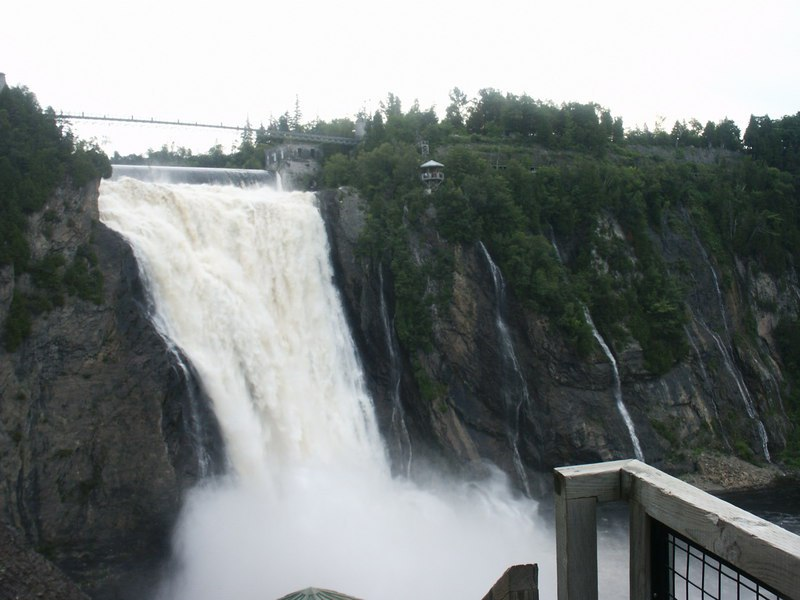
\includegraphics[height=.9\textheight]{images/0116_falls_and_rock}
\end{center}
\end{frame}

\begin{frame}[fragile]
\frametitle{Waterfall Model: The Ideal}

\begin{center}
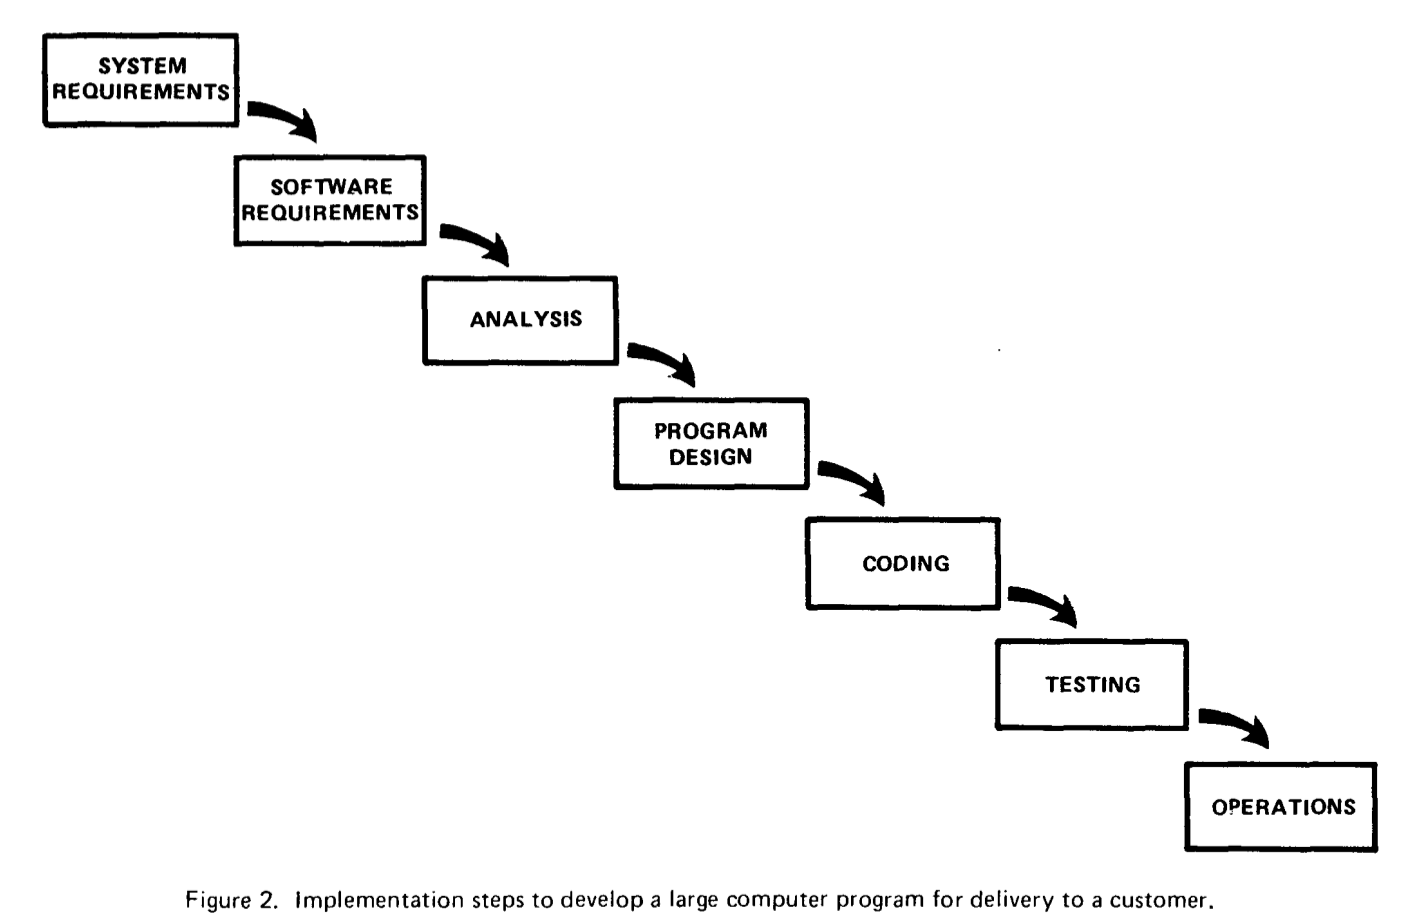
\includegraphics[height=.7\textheight]{images/classic-waterfall.png}
\end{center}

\end{frame}

\begin{frame}
\frametitle{Waterfall Model}

\begin{changemargin}{1cm}
Highly sequential: stages do not overlap.\\
Project moves onto the next stage following reviews.\\[1em]

Advantages: 
\begin{enumerate}
\item fixes customer requirements early\\ (hopefully the right requirements); 
\item could identify
problems early in the design process, when changes are less expensive.
\end{enumerate}
~\\[1em]
Disadvantages: 
\begin{enumerate}
\item working blind---don't see any
software until the end of the implementation stage (a big deal!);
\item changes late in development imply wasted work.
\end{enumerate}

\end{changemargin}
\end{frame}

\begin{frame}
\frametitle{Waterfall Model: Dealing with Change}

\begin{center}
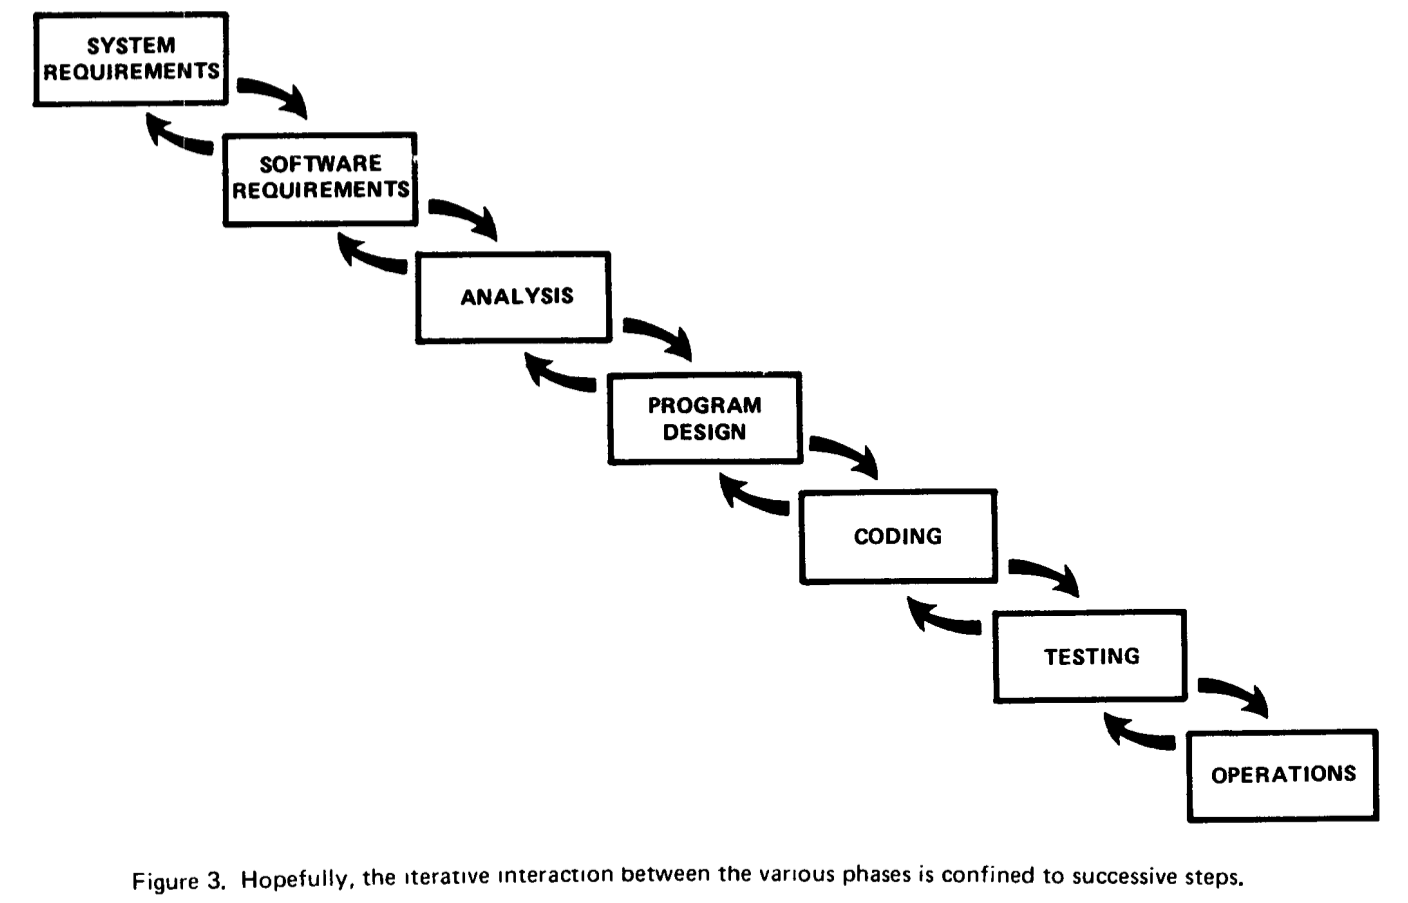
\includegraphics[height=.7\textheight]{images/more-ideal-iteration}
\end{center}

\end{frame}

\begin{frame}
\frametitle{Waterfall Model: More Likely Scenario}

\begin{center}
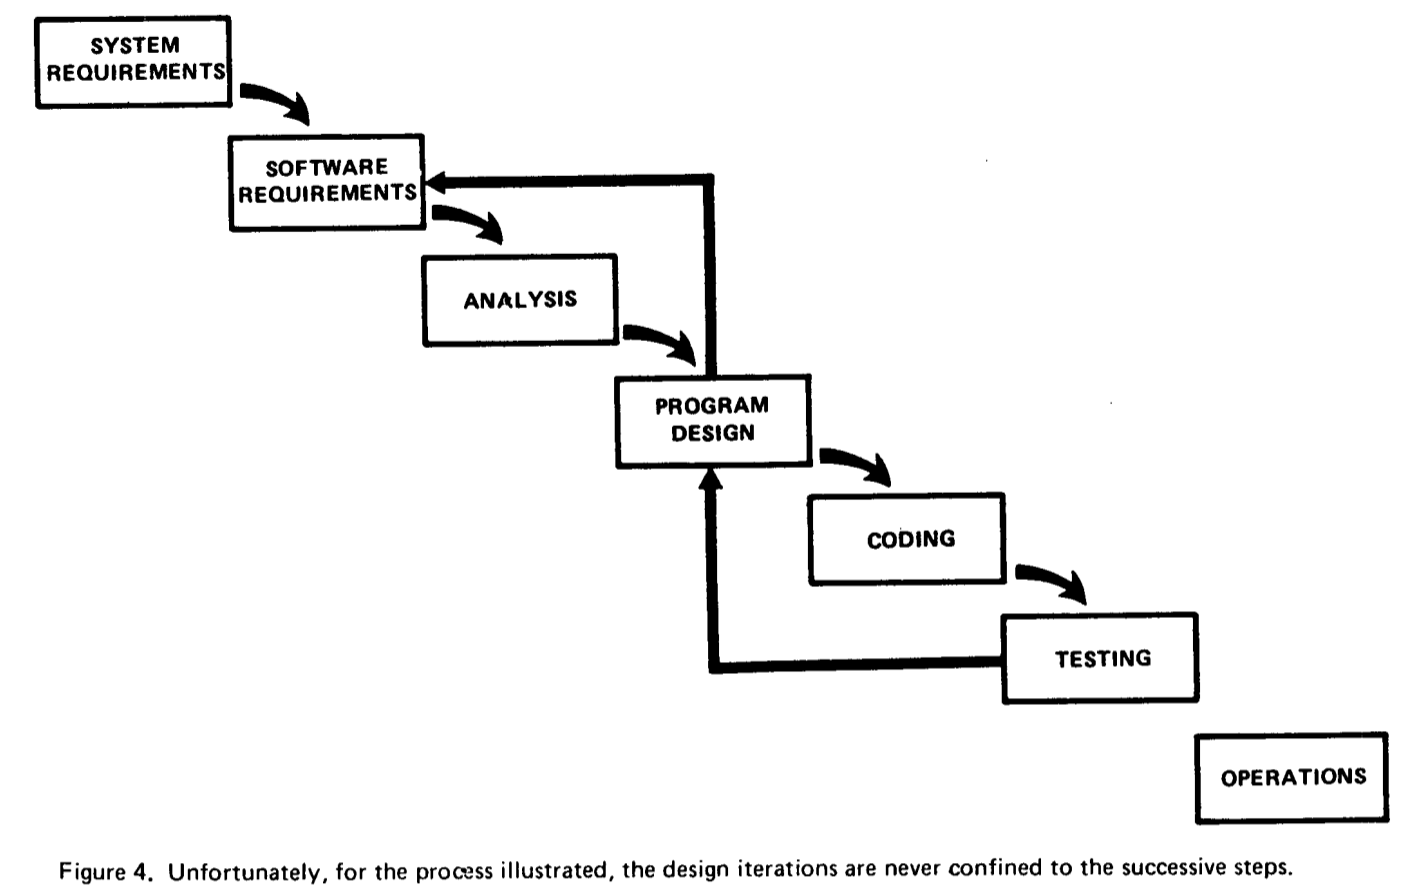
\includegraphics[height=.7\textheight]{images/less-ideal-iteration}
\end{center}

\end{frame}

\begin{frame}
\frametitle{Waterfall Model}

\begin{changemargin}{1cm}
It's a strawman.
% http://upload.wikimedia.org/wikipedia/commons/3/38/McKinley_Destroys_Imperialism_Straw_Man.jpg

\begin{center}
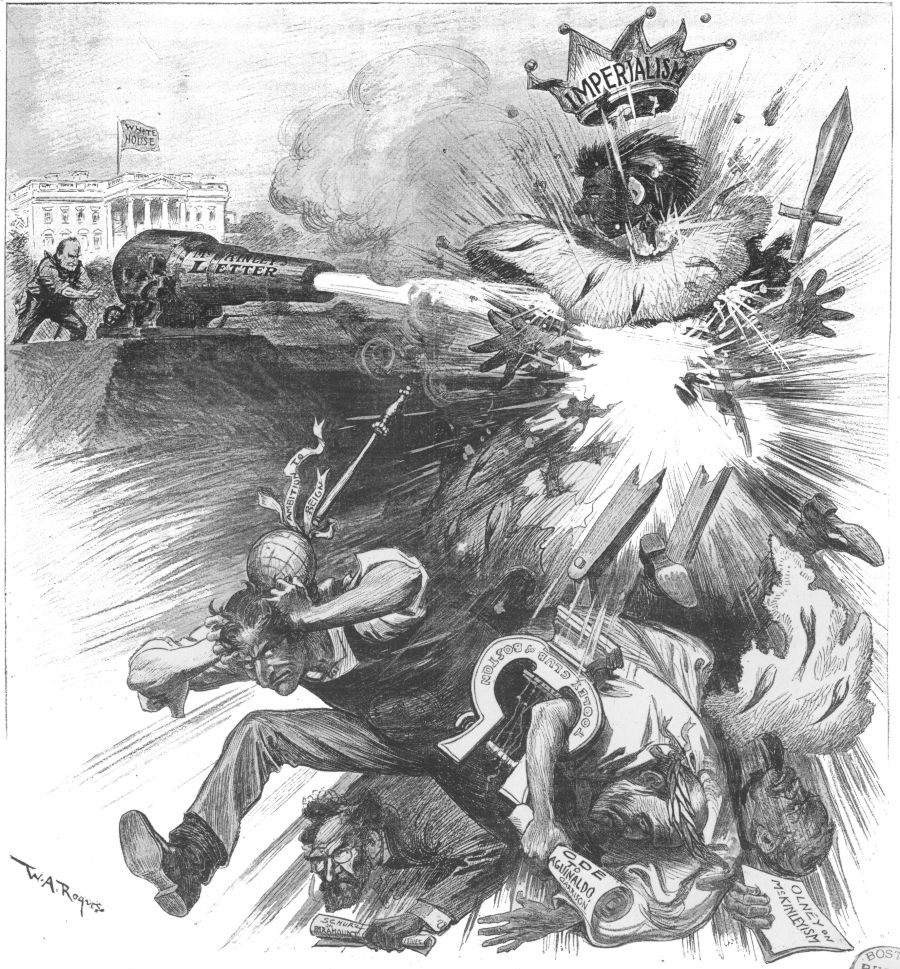
\includegraphics[height=.7\textheight]{images/McKinley_Destroys_Imperialism_Straw_Man}
\end{center}
{\hfill \scriptsize Harper's Weekly, September 22, 1900, p. 881.}

No one seriously advocates this model.\\
\end{changemargin}
\end{frame}

\begin{frame}
\frametitle{Concurrent Engineering}

%  http://upload.wikimedia.org/wikipedia/commons/thumb/2/21/Sashimi.jpg/800px-Sashimi.jpg

Also known as sashimi model:
\begin{center}
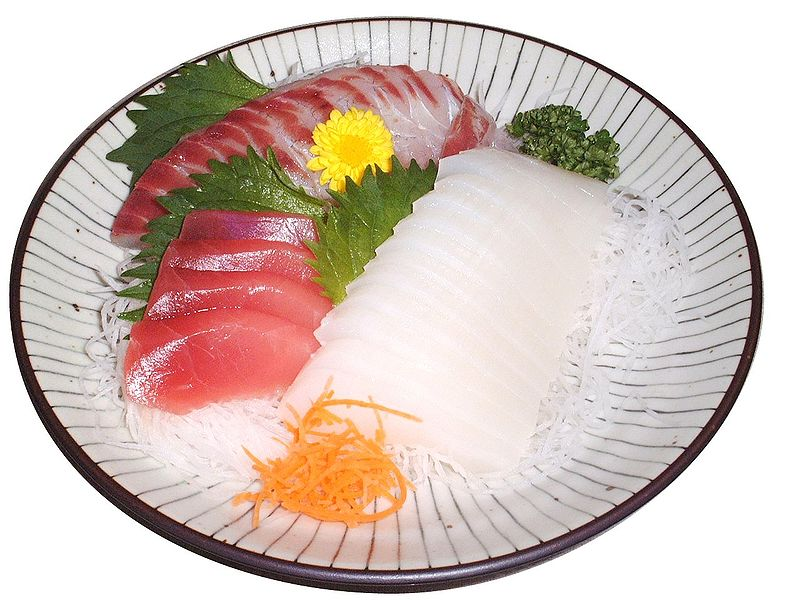
\includegraphics[height=.7\textheight]{images/800px-Sashimi}
\end{center}
{\hfill \scriptsize Wikimedia commons, credit Suguri\_F}

\end{frame}

\begin{frame}
\frametitle{Concurrent Engineering: a More Realistic Waterfall}

\begin{changemargin}{1cm}
Don't wait on the previous stage to finish:\\
start the next stage as soon as possible.\\
\qquad (hence, sashimi).

\begin{center}
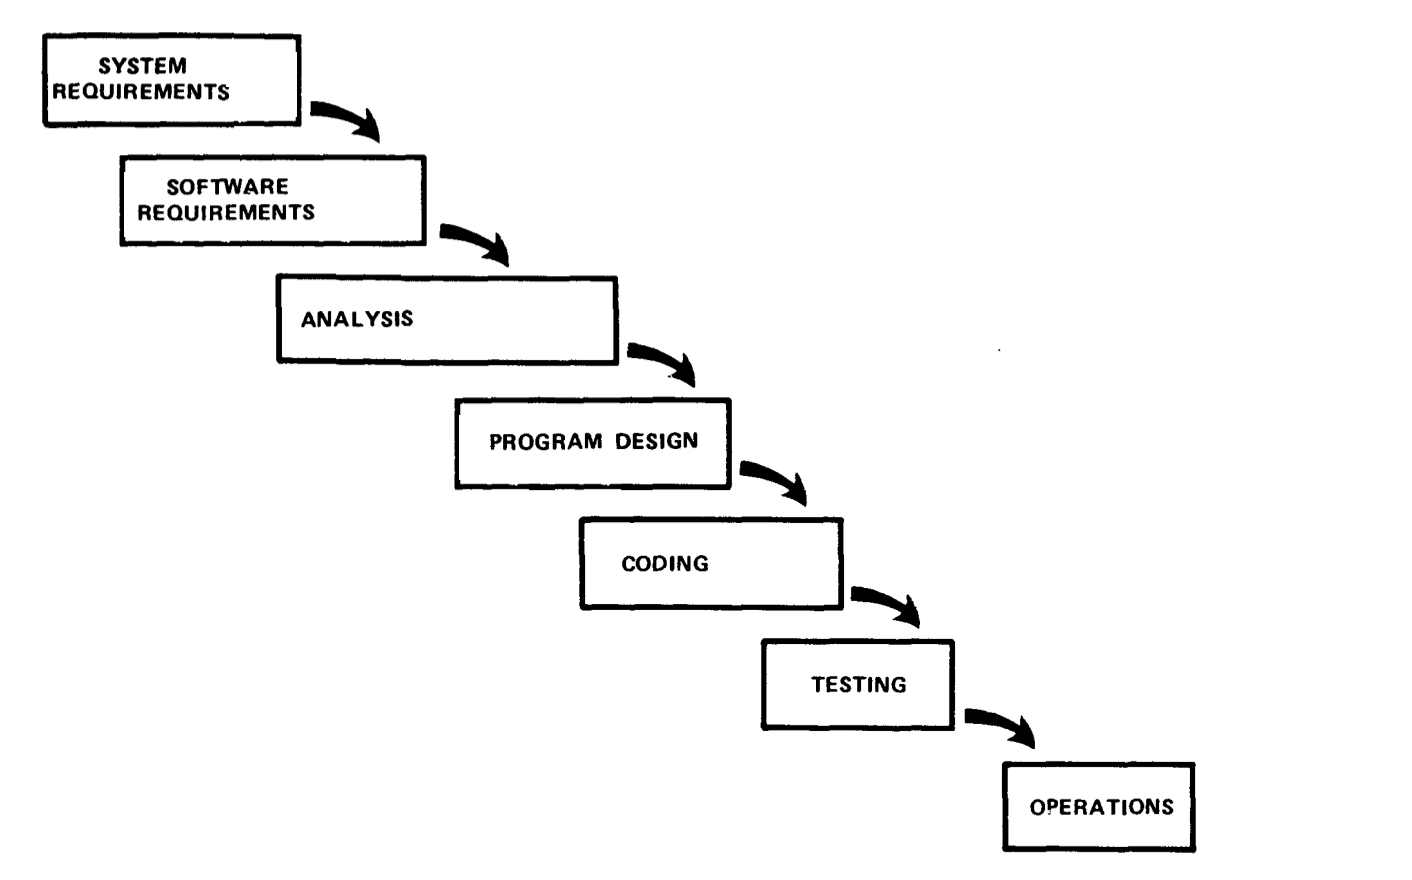
\includegraphics[height=.6\textheight]{images/concurrent-engineering}
\end{center}

Key idea: \structure{Why wait?}\\
Using a product is a good way to refine it.

\end{changemargin}
\end{frame}

\begin{frame}
\frametitle{Concurrent Engineering: Advantages and Disadvantages}
\begin{changemargin}{1cm}
Advantages: 
\begin{enumerate}
\item because you don't need to write down every last
  (irrelevant) detail, might need less documentation; 
\item projects need not be subdivided into smaller projects; 
\item testing and use may reveal problems earlier.
\end{enumerate}
~\\[1em]
Disadvantages: 
\begin{enumerate}
\item milestones may be more ambiguous; 
\item progress is more difficult to track: \\
\qquad how done is stage $x$, anyway?; 
\item poor
  communication more likely to lead to disaster.
\end{enumerate}


\end{changemargin}
\end{frame}

\begin{frame}
\frametitle{The V-Model}

\begin{changemargin}{1cm}
Take Waterfall and link the stages horizontally.

\begin{center}
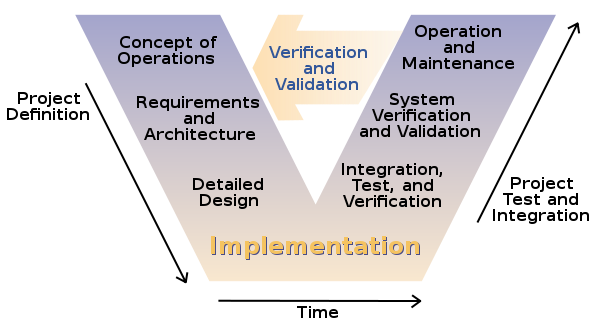
\includegraphics[height=.5\textheight]{images/vmodel.png}
\end{center}

Key idea: \structure{Make links explicit}
\end{changemargin}
\end{frame}

\begin{frame}
\frametitle{V-Model Advantages and Disadvantages}
\begin{changemargin}{1cm}
Advantages: 
\begin{enumerate}
\item Another attempt at a more realistic description of Waterfall
\item Otherwise the same as the any other variant of Waterfall
\end{enumerate}
~\\[1em]
Disadvantages: 
\begin{enumerate}
\item the same as any other variant of Waterfall
\end{enumerate}

\end{changemargin}
\end{frame}

\begin{frame}
\frametitle{Spiral Model}

\begin{center}
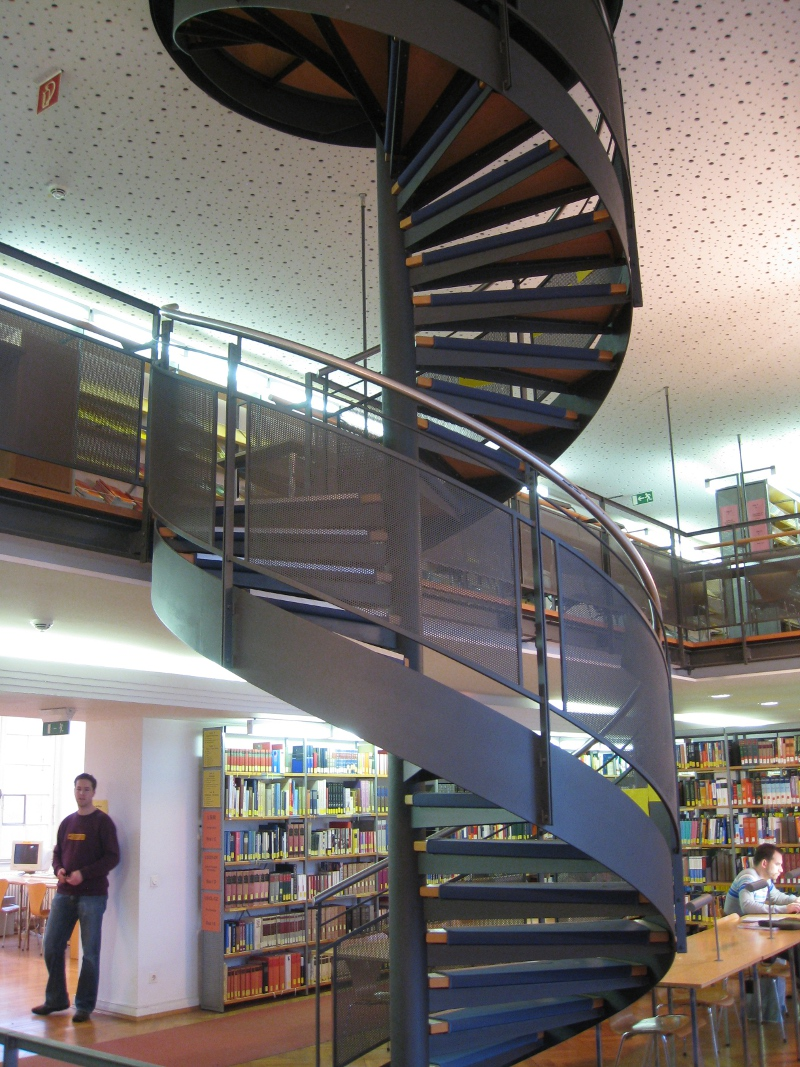
\includegraphics[height=.6\textheight]{images/3821_spiral_staircase_in_library}
\end{center}

\begin{changemargin}{1cm}
Iterate the waterfall.
\end{changemargin}

\end{frame}

\begin{frame}
\frametitle{Spiral Model: Diagram}

% http://en.wikipedia.org/wiki/File:Spiral_model_%28Boehm,_1988%29.svg

\begin{center}
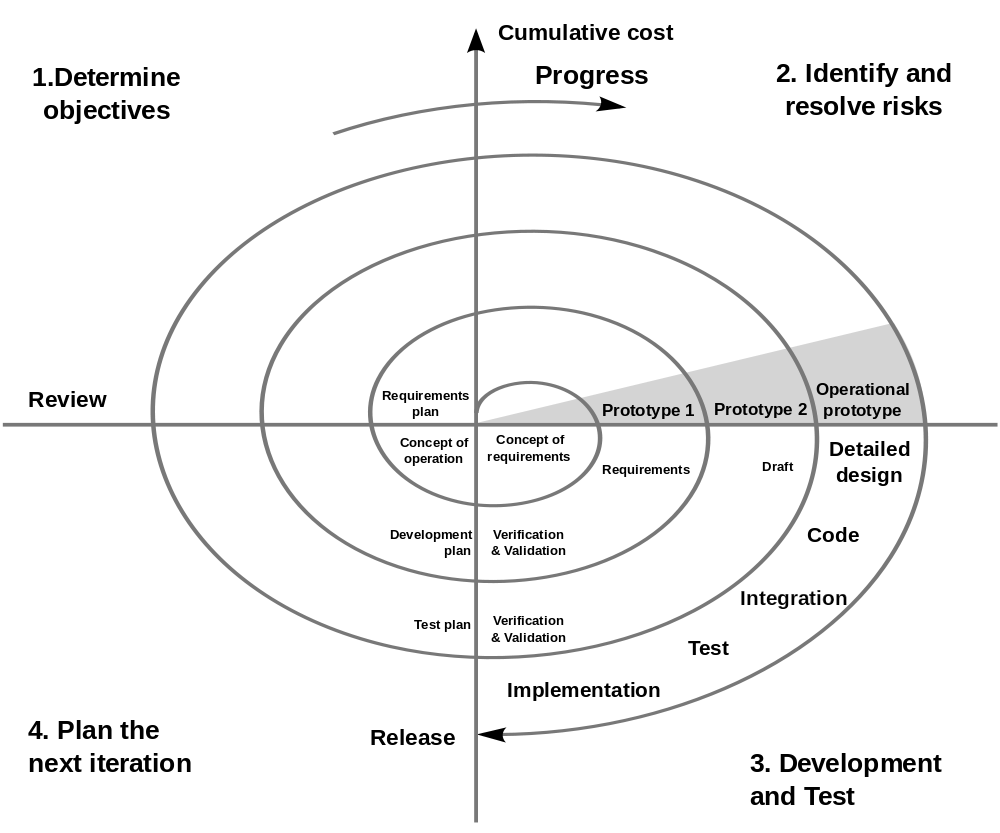
\includegraphics[height=.7\textheight]{images/spiral-boehm.png}
\end{center}
\end{frame}

\begin{frame}
\frametitle{Spiral Model: Explanation}
\begin{changemargin}{1.5cm}

Iterate through stages, in order, until you get to
a satisfactory solution. \\[1em]

Projects split into smaller
sub-projects; \\
each iteration corresponds to a smaller project.\\[1em]

Iterate many times. \\[2em]

Not all stages require equal effort: \\
testing often harder than coding.\\[1em]

Risk-oriented model; \\
each sub-project addresses
one or more risks (riskiest first), \\
until all of the major risks
have been addressed. 
\end{changemargin}
\end{frame}

\begin{frame}
\frametitle{Spiral Model: Advantages and Disadvantages}
\begin{changemargin}{1cm}
Advantage:
\begin{itemize}
\item addresses the biggest risks first, \\
when changes are least expensive; 
\item progress visible to customer \& management.
\end{itemize}
~\\[1em]
Disadvantage:
\begin{itemize}
\item some projects don't have clearly identifiable
sub-projects with verifiable milestones.
\end{itemize}
\end{changemargin}
\end{frame}

\begin{frame}
\frametitle{Summary}
\begin{changemargin}{1cm}

In industry: accepted that Waterfall is obsolete \\
\hfill ...if not outright harmful.

Iterations are the accepted method for development.

Now: we'll look at iterations in more detail.

\end{changemargin}
\end{frame}

\part{Software Lifecycle Tactics}
\frame{\partpage}

\begin{frame}
\frametitle{Some Software Lifecycle Tactics}

\begin{changemargin}{2cm}
\begin{itemize}
\item Cowboy Coding
\item Scrum
\item Test-Driven Development
\item Behaviour-Driven Development
\item Kanban
\end{itemize}
~\\

\end{changemargin}
\end{frame}


\begin{frame}
\frametitle{Scrum Model}

\begin{center}
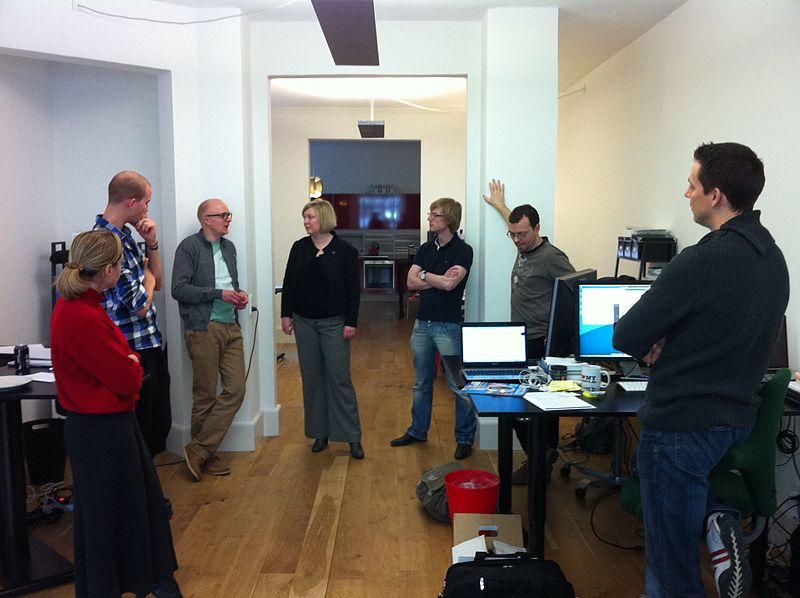
\includegraphics[height=.7\textheight]{images/sprint-meeting.jpg}
\end{center}

Short iterations.
%{\small \url{http://en.wikipedia.org/wiki/File:Daily_sprint_meeting.jpg}}

\end{frame}


\begin{frame}
\frametitle{Scrum Model: Diagram}
\begin{center}
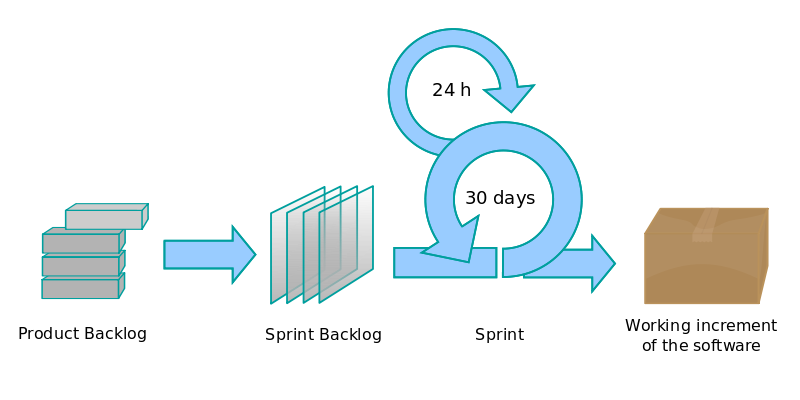
\includegraphics[width=0.9\textwidth]{images/scrum.png}
\end{center}

\end{frame}

\begin{frame}
\frametitle{Scrum Model: Explanation}
\begin{changemargin}{1.5cm}

Break the work down into a series of short iterations. \\
Usually around 30 days. \\
~\\
Strictly defined iterations (in terms of features and time).\\
~\\
Daily meetings to co-ordinate.\\
~\\
Collect feedback for the next sprint.\\

\end{changemargin}
\end{frame}

\begin{frame}
\frametitle{Scrum Model: Advantages and Disadvantages}
\begin{changemargin}{1.5cm}

Advantages:
\begin{enumerate}
	\item Short iterations mean lots of opportunities for input and feedback. 
	\item Daily meetings mean lots of co-ordination between team members. 
	\item It encourages breaking the software down into manageable units.
\end{enumerate}

Disadvantages:
\begin{enumerate}
	\item It does not scale well to large teams.
	\item Daily meetings can result in excessive overhead.
	\item At the sprint deadline, development ends whether the code is finished or not!
\end{enumerate}

\end{changemargin}
\end{frame}


\begin{frame}
\frametitle{Test-Driven Development}

\begin{center}
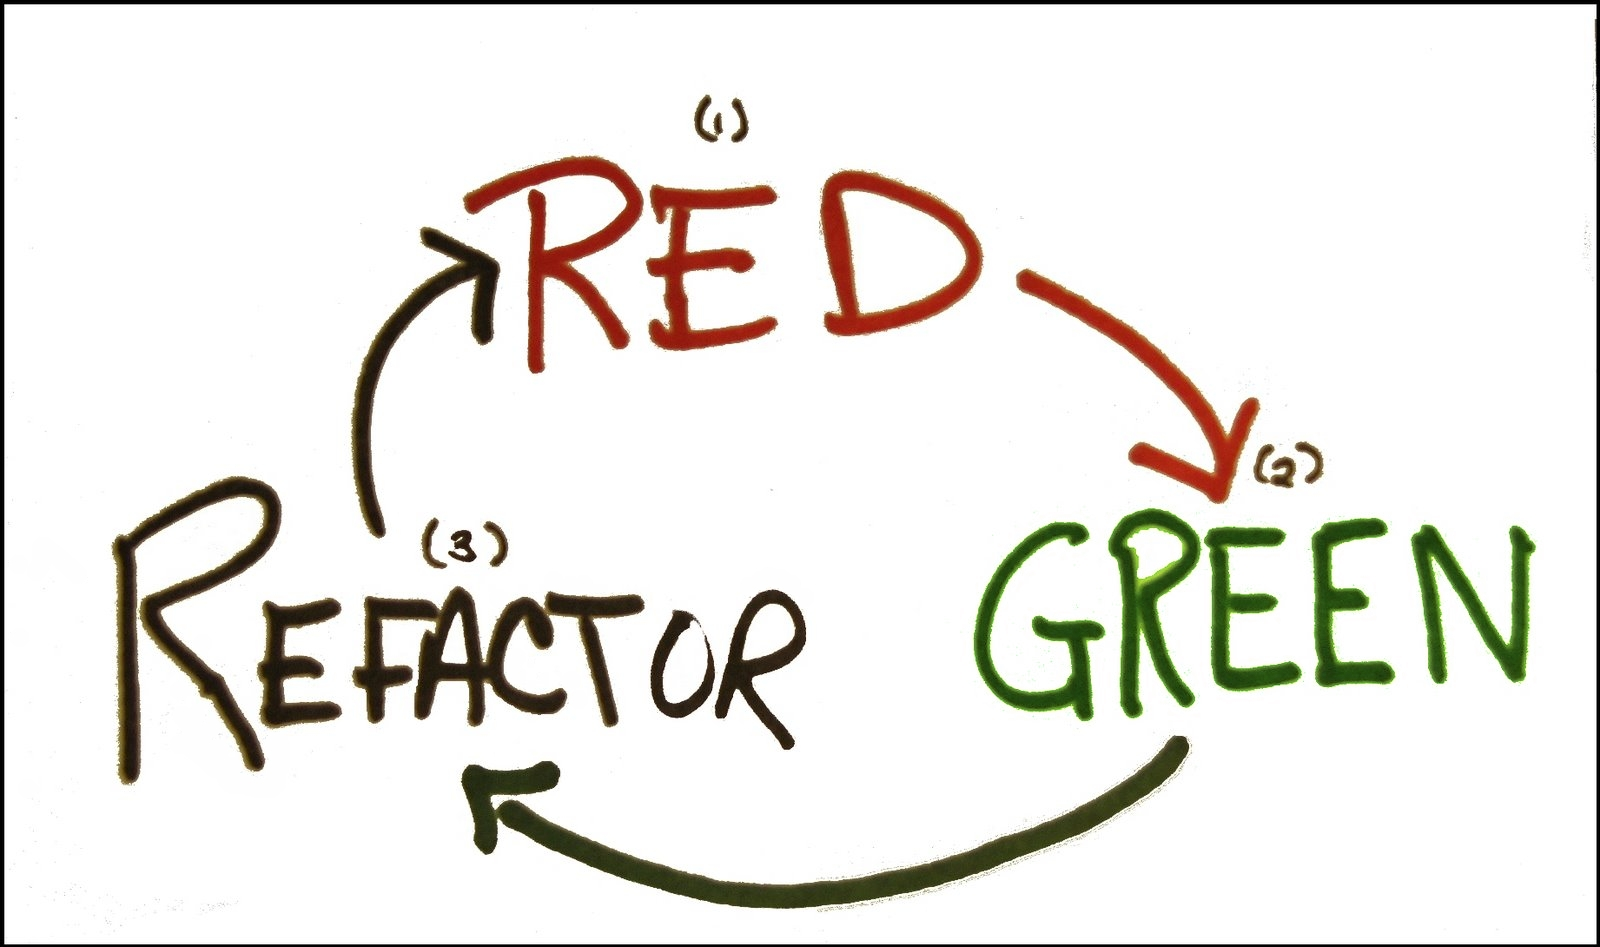
\includegraphics[height=.7\textheight]{images/redgreenrefactor.jpeg}
\end{center}

Write the tests first.
%{\small \url{http://www.schiffhauer.com/wp-content/uploads/2013/04/d1d5e9cc98c64375e99e35b1bab596e1.jpeg}}

\end{frame}


\begin{frame}
\frametitle{TDD: Diagram}
\begin{center}
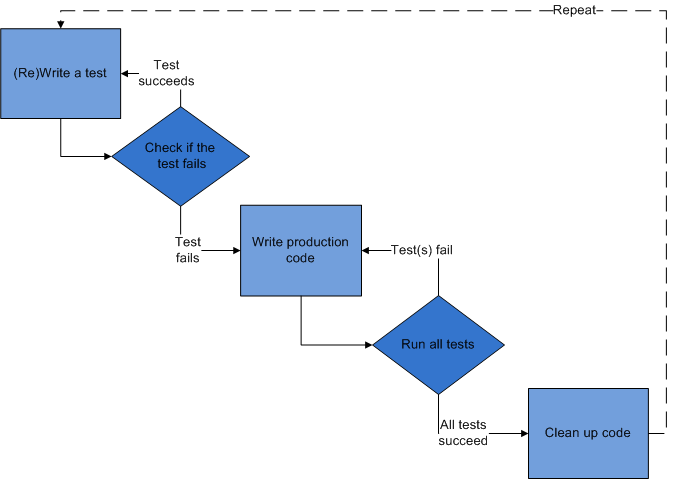
\includegraphics[width=0.9\textwidth]{images/tdd.png}
\end{center}

\end{frame}

\begin{frame}
\frametitle{TDD: Explanation}
\begin{changemargin}{1.5cm}

Write the tests first, then the code.\\~\\

Create a test for a new feature. It should fail.\\~\\

Develop the code until the test passes.\\~\\

Then, refactor (clean up) the code\\~\\

More time spent on testing, with the goal of saving time in the long run.

\end{changemargin}
\end{frame}

\begin{frame}
\frametitle{TDD: Advantages}
\begin{changemargin}{1.5cm}

Advantages:
\begin{enumerate}
	\item This model emphasizes testing in a way that other models do not. 
	\\
	When time is short and the product needs to be released, testing is usually cut... TDD prevents this.
	\item More code will be covered by the tests.
	\item It encourages breaking the software down into testable units.
\end{enumerate}

\end{changemargin}
\end{frame}

\begin{frame}
\frametitle{TDD: Disadvantages}
\begin{changemargin}{1.5cm}

Disadvantages:
\begin{enumerate}
	\item An error in the code may be undetected because of a similar error in the unit test.
	\item Not everything is testable.
	\item TDD focuses only on unit tests, and this is not the only kind of testing.
	\item Redundant or inflexible tests.
	\item Tendency to disable broken tests or implement a quick change to ``fix'' the test.
	\item Passing tests are not the same thing as functioning, useful software.
\end{enumerate}

\end{changemargin}
\end{frame}

\begin{frame}
\frametitle{About Extreme Programming (XP)}
\begin{changemargin}{2cm}
Another software lifecycle model, but an outlier.\\

Most resembles spiral model, but scaled down \& more agile.\\[1em]

Agile: Take ``good'' parts of good programming practice
\begin{center}
(e.g. reviews, testing)
\end{center}
and ``crank up all the knobs to 10''.\\[1em]

Leave everything else behind.\\[1em]

XP is one of several agile methodologies:\\
all attempt to be less bureaucratic than the traditional
``heavyweight'' methodologies. 

\end{changemargin}
\end{frame}

% up to 11:
% http://www.youtube.com/watch?v=UeOXsA8sp_E

\begin{frame}
\frametitle{XP Values}
\begin{changemargin}{2cm}
XP comes with a set of values:
\begin{itemize}
\item Communication\\[2em]
% Work together. Includes pair programming. Face-to-face communication.
% Workspaces to support collaboration. Don't generate paperwork.
% Share knowledge.
\item Simplicity\\[2em]
% don't do more than you need to. Take small, simple steps to goal.
% You Ain't Gonna Need It. Requires refactoring later.
\item Feedback\\[2em]
% Get feedback from system (unit tests), from client (functional/acceptance 
% tests), from the team (time estimates). Demo working software.
\item Courage\\[2em]
% Code for today, not tomorrow.
% Refactor when necessary, don't be scared.
% Throw code away when necessary.
% Work together to avoid failure and not fear it.
\item Respect\\[2em]
% Respect contributions of other team members (devs and customers)
% Management respects judgment of programmers.
% Don't break the build or waste others' time.
\end{itemize}
\end{changemargin}
\end{frame}

\begin{frame}
\frametitle{XP: Basic Activities}
\begin{changemargin}{2cm}
\Large
Four basic activities: 
\begin{itemize}
\item coding;
\item testing;
\item listening; and
\item designing.
\end{itemize}
\end{changemargin}
\end{frame}

\begin{frame}
\frametitle{XP: Coding}
\begin{changemargin}{2cm}

\structure{The code is central.}\\
(not requirements docs, specifications)\\[1em]

XP: try to get working code out as soon as possible.\\
(even code with limited scope).\\[1em]

Programmers produce code in pairs.\\[1em]

Code runs, but also serves as main communication and experimentation medium.
\end{changemargin}
\end{frame}

\begin{frame}
\frametitle{XP: Testing}
\begin{changemargin}{2cm}

XP advocates test-driven development, as we've seen: \\
\begin{itemize}
\item first, write the test;
\item make sure test fails;
\item implement simplest possible solution;
\item make sure test passes.
\end{itemize}

Code must always pass all of the unit tests.\\[1em]

Also, acceptance tests (more below).
\end{changemargin}
\end{frame}

\begin{frame}
\frametitle{XP: Listening}
\begin{changemargin}{2cm}

General problem: \\
\qquad \structure{Is the code doing the right thing?}\\[1em]

XP solution: Acceptance tests,\\
created by on-site customer.\\[1em]

Also: developers must listen to business people and~vice-versa.
\end{changemargin}
\end{frame}

\begin{frame}
\frametitle{XP: Designing}
\begin{changemargin}{2cm}

No big up-front design.\\[1em]

Create a design incrementally by constantly re-factoring code as
written (more later).
\end{changemargin}
\end{frame}

\begin{frame}
\frametitle{XP: Advantages}

\begin{changemargin}{1cm}
Can help avoid getting caught in bureaucratic tarpits;\\[1em]
When you have a good team, XP should deliver good results:\\
\qquad get simpler designs which solve the appropriate problems; \\
\qquad respond well to changes in requirements.
\end{changemargin}
\end{frame}

\begin{frame}
\frametitle{XP: Disadvantages and Controversies}

\begin{changemargin}{1cm}
Per Kent Beck: \\
\quad XP works best when one uses all of the practices
together. \\[1em]

Some of the practices can work alone, \\
like test-driven
development. \\[1em]

Others may not work as well in 
isolation.\\
\qquad (``... ring of poisonous snakes, daisy-chained together.'') \\[2em]

XP tends to work best with smaller-sized groups \\ \qquad ($< 12$ members).\\
Lack of up-front design and requirements specifications can be
worrisome.
\end{changemargin}
\end{frame}


\begin{frame}
\frametitle{Kanban}

\begin{changemargin}{1cm}
\textit{Kanban} -- Japanese word for ``Visual Card''

Comes from Toyota's car manufacturing process.

Support non-centralized production control: \\
	\quad work is pulled, not pushed.
\end{changemargin}
\end{frame}


\begin{frame}
\frametitle{Kanban: Identify Bottlenecks}

\begin{changemargin}{1cm}
\alert{Bottleneck}: Stage of production that limits rate of output.
\begin{center}
	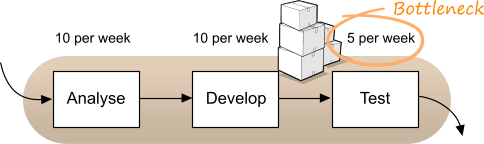
\includegraphics[width=0.7\textwidth]{images/bottleneck-inventory.png}
\end{center}

Temptation: cut corners to reduce backlog.

\end{changemargin}
\end{frame}

\begin{frame}
\frametitle{Kanban: Cards and Board}
\begin{changemargin}{1cm}

Physical or virtual cards represented on a board that has categories.

A card represents a unit of work.

Cards cannot advance until there is space farther along.

\end{changemargin}
\end{frame}



\begin{frame}
\frametitle{Kanban Board Example}
\begin{center}
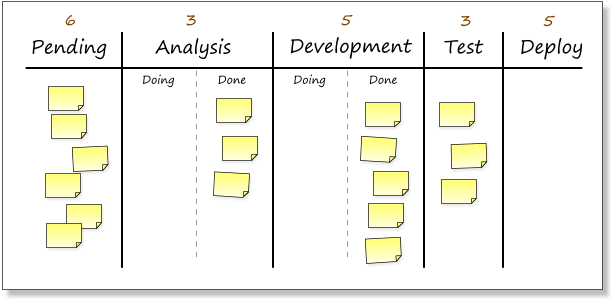
\includegraphics[width=0.9\textwidth]{images/kanban-board-1.png}
\end{center}
\mnote{Developers and analysts can't take on any more work until the testers finish some of the items on their plate.}
\end{frame}

\begin{frame}
\frametitle{Kanban Board Example}
\begin{center}
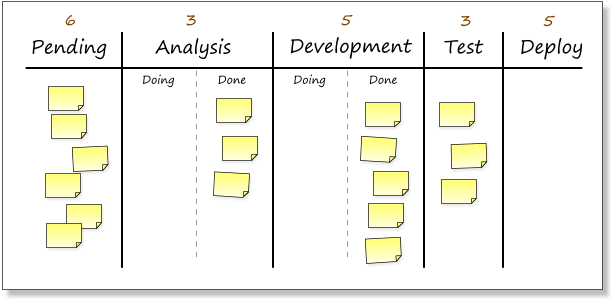
\includegraphics[width=0.9\textwidth]{images/kanban-board-1.png}
\end{center}

Backlog at the ``Test'' stage. How to address this? \mnote{Hire more testers? Have analysts and developers help with testing?}

\end{frame}

\begin{frame}
\frametitle{Kanban Board Example}
\begin{center}
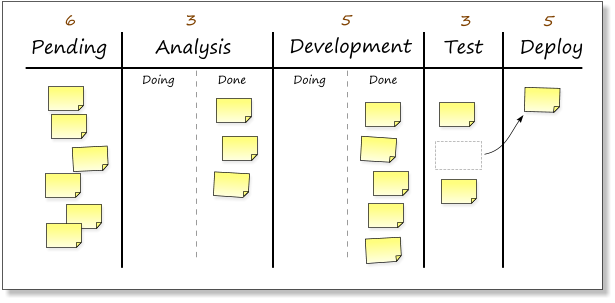
\includegraphics[width=0.9\textwidth]{images/kanban-board-2.png}
\end{center}
Testers finish a feature and it moves to ``deploy''...
\end{frame}

\begin{frame}
\frametitle{Kanban Board Example}
\begin{center}
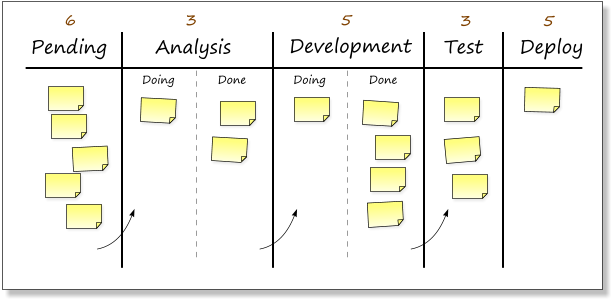
\includegraphics[width=0.9\textwidth]{images/kanban-board-3.png}
\end{center}
... and now the other stages may advance.
\end{frame}

\begin{frame}
\frametitle{Kanban: Advantages \& Disadvangages}
\begin{changemargin}{1cm}

Advantages:
\begin{itemize}
	\item Make bottlenecks visible.
	\item Prevent overloading of any stage.
	\item Estimation is not present. \mnote{No time wasted on that}
\end{itemize}

Disadvantages:
\begin{itemize}
	\item Stoppage in one part of the process can stop many others \mnote{should developers just sit there with nothing to do because analysis is delayed?}
	\item Estimation can be valuable.
	\item No commitment of features to versions.
\end{itemize}

\end{changemargin}
\end{frame}



\end{document}
